\documentclass[10pt]{article}
%\documentclass[10pt,fullpage]{article}
%\usepackage[T1]{fontenc}
%\usepackage[latin9]{inputenc}
%\bibliographystyle{plain}
\usepackage{helvet}
%\usepackage{times}
\usepackage{epsfig}
\usepackage[small,compact]{titlesec}
\usepackage[reqno]{amsmath}
\usepackage{color}
\usepackage{fancybox}
\bibliographystyle{plain}
\usepackage[super]{natbib}
\setlength{\evensidemargin}{0in}
%\setlength{\evensidemargin}{-0.15in}
%\setlength{\oddsidemargin}{-0.15in}
%\setlength{\oddsidemargin}{0in}
%\setlength{\marginparwidth}{0.0in}
%\setlength{\textwidth}{6.50in}
%\setlength{\textheight}{9.0in}
%\setlength{\topmargin}{0.55in}
%\setlength{\topmargin}{0in}
%\setlength{\headheight}{0in}
%\setlength{\headsep}{0in}
%\setlength{\columnsep}{0.20in}
\pagestyle{plain}
\makeatletter
%%%%%%%%%%%%%%%%%%%%%%%%%%%%%% User specified LaTeX commands.



\usepackage{epsfig,longtable}
%\usepackage{fullpage,doublespace}
%\usepackage{psfrag}
%\usepackage{genres}
%\usepackage{times}
%\usepackage{latexsym}
%\usepackage{fancybox,subfigure}
\usepackage[normalem]{ulem}
%\usepackage{normalem}
%\bibliographystyle{plain}
%\usepackage{amsmath}
%\usepackage{mathrsfs}
%\usepackage{algorithmic}
%\usepackage{tweaklist}

\newcommand{\captionfonts}{\small}
\usepackage{float}
\floatstyle{plain}
\newfloat{supplementalfigure}{thp}{sup}
\floatname{supplementalfigure}{Figure S\hspace{-3pt}}
\newfloat{supplementaltable}{thp}{sup}
\floatname{supplementaltable}{Table S\hspace{-3pt}}

%%%
\newtheorem{problem}{Problem}

%\makeatletter
%\def\@cite#1#2{$^{\mbox{\tiny #1\if@tempswa , #2\fi}}$}
%\makeatother

\makeatletter  % Allow the use of @ in command names
\long\def\@makecaption#1#2{%
  \vskip\abovecaptionskip
  \sbox\@tempboxa{{\captionfonts #1: #2}}%
  \ifdim \wd\@tempboxa >\hsize
    {\captionfonts #1: #2\par}
  \else
    \hbox to\hsize{\hfil\box\@tempboxa\hfil}%
  \fi
  \vskip\belowcaptionskip}

%\def\aligntop#1{\setbox\@tempboxa \hbox{#1}%
%                \@tempdima=\ht\@tempboxa%
%                \advance\@tempdima-\ht\strutbox%
%                \leavevmode\lower\@tempdima\box\@tempboxa}

\makeatother   % Cancel the effect of \makeatletter

\setlength{\topmargin}{-0.5in}
\usepackage{latexsym}
\setlength{\columnsep}{0.5cm} 
\setlength{\oddsidemargin}{-0cm}
\setlength{\evensidemargin}{-0cm} 
\setlength{\textwidth}{6.8in}
\setlength{\textheight}{8.7in}

\newcommand{\old}[1]{}
\newcommand{\match}{\stackrel{M}{=}}
\newcommand{\ncite}[1]{$^{\mbox{\tiny \cite{#1}}}$}
%\newcommand{\nncite}[1]{\cite{#1}}
\newcommand{\frags}{{\cal F}}
\newcommand{\snips}{{\cal S}}
\newcommand{\A}{{\tt A}}
\newcommand{\B}{{\tt B}}
\newcommand{\gap}{{\tt -}}
\newcommand{\ideas}{\vskip 0.6cm {\bf IDEAS:\ }}
\newcommand{\motivation}{\vskip 0.6cm {\bf MOTIVATION:\ }}
\newcommand{\mcost}[2]{#1 #2}
\newcommand{\ali}{$\mbox{ }$\hspace{0.1in}}
\newcommand{\acomment}[1]{\hspace{1in}\#{\em #1}}
\newcommand{\beqn}{\begin{equation}}
\newcommand{\eeqn}{\end{equation}}
\newcommand{\comment}[1]{******* {\em #1} *******}
%\newcommand{\LtoN}[1]{\parallel #1 \parallel_{2}}
\newcommand{\LtoN}[1]{\left\Vert {#1} \right\Vert}
\newcommand{\Ntr}[1]{\frac{\vecbf{#1}-P_{#1}}{\sqrt{P_{#1}P_{\bar{#1}}}}}

\newcommand{\BIN}[1]{\left\langle{#1}\right\rangle}
\newcommand{\ABS}[1]{\left|{#1}\right|}
\newcommand{\FLOOR}[1]{\left\lfloor{#1}\right\rfloor}
\newcommand{\CEIL}[1]{\left\lceil{#1}\right\rceil}
%\newcommand{\SET}[1]{\left\{{#1}\right\}}
\newcommand{\SET}[1]{\{{#1}\}}
\newcommand{\Rapid}{{\sc Rapid}}
\newcommand{\subbox}[1]{\mbox{\footnotesize #1}}

\newcommand{\captionsize}{\footnotesize}
\newcommand{\mecca}{HapCUT$\:$}
%\newcommand{\vecbf}[1]{{\bf #1}}
\let\vecbf\boldsymbol
%\newcommand\vecbf[1]{\boldsymbol{\vec #1}}
%%%%%%%%%%%%%% Figure within a box
\newenvironment{boxfig}[1]{\fbox{\begin{minipage}{\linewidth}
                        \vspace{1em}
                        \makebox[0.025\linewidth]{}
                        \begin{minipage}{0.95\linewidth}
                        #1
\end{minipage}
                        \end{minipage}}}

\newcommand{\proc}[1]{\ensuremath{\mbox{\sc #1}}}

\newcommand{\MST}{\ensuremath{\mathit{MST}}}
\newcommand{\dist}{\ensuremath{\mathrm{dist}}}
\newcommand{\TG}[2]{\ensuremath{\mathit{#1}^{(#2)}}}
\newcommand{\CC}{\ensuremath{\mathcal{CC}}}
\newcommand{\psubs}{\stackrel{\subset}{+}}
\newcommand{\rs}{\ensuremath{\mathit{R_s}}}
\newcommand{\MEC}{\ensuremath{\mathit{MEC}}}
\newcommand{\Prob}{\ensuremath{\mbox{Pr}}}
\newcommand{\Exp}{\ensuremath{\mbox{E}}}

%%%%%%%%%%%%%%%%%%%%%%%%%%%%%  THEOREM-LIKE ENVIRONMENTS

\newtheorem{THEOREM}{{\bf  Theorem}}
\newenvironment{theorem}{\begin{THEOREM} \hspace{-.85em}  {\bf :} }%
                        {\end{THEOREM}}
\newtheorem{LEMMA}[THEOREM]{Lemma}
\newenvironment{lemma}{\begin{LEMMA} \hspace{-.85em} {\bf :} }%
                      {\end{LEMMA}}
\newtheorem{COROLLARY}[THEOREM]{Corollary}
\newenvironment{corollary}{\begin{COROLLARY} \hspace{-.85em} {\bf :} }%
                          {\end{COROLLARY}}
\newtheorem{PROPOSITION}[THEOREM]{Proposition}
\newenvironment{proposition}{\begin{PROPOSITION} \hspace{-.85em} {\bf :} }%
                            {\end{PROPOSITION}}
\newtheorem{CLAIM}[THEOREM]{Claim}
\newenvironment{claim}{\begin{CLAIM} \hspace{-.85em} {\bf :} }%
                      {\end{CLAIM}}
\newtheorem{OBSERVATION}[THEOREM]{Observation}
\newenvironment{Observation}{\begin{OBSERVATION} \hspace{-.85em} {\bf :} }%
                      {\end{OBSERVATION}}
\newtheorem{DEFINITION}{Definition}
\newenvironment{definition}{\begin{DEFINITION} \hspace{-.85em} {\bf :} }%
                           {\end{DEFINITION}}
\newcommand{\QED}{\hfill$\clubsuit$ \vskip 0.1cm}
\newenvironment{proof}{\noindent {\bf Proof:} \hspace{.677em}}{\QED}


\begin{document}

\title{\vspace{-1in} Layering for Genomics: iDASH Milestones}
\author{Vineet Bafna\thanks{CSE 4218, Univ. California, San Diego. \{vbafna,gvarghese\}@cs.ucsd.edu} \and George Varghese$^*$}
\date{}
\maketitle
\section{Executive summary}
As sequencing costs drop and DNA sequences become part of every
patient record to enable personalized medicine, it will become
essential to have engineered (as opposed to ad hoc) methods to
efficiently manage the large amount of genetic data.  We consider the
imminent future where individual (\emph{donor}) genomic sequences will
be generated as sub-chromosomal fragments. We assume that most queries
of this data will involve the genetic variations between the donor
genome and a standard reference.  We propose a general vision of
layered software for genomics (inspired by other computer systems such
as the Internet and databases) to allow applications (such as
pharmocogenomics and cancer genomics) to efficiently query, index and
compress this vast genomic database.  In the context of this {\em
  general} vision, we have two {\em specific} objectives for this
short proposal.

\begin{itemize}
\item We propose continued collaborations with School of Medicine on
  the development of tools for analyzing genomic data.
\item We propose to develop and publish a layered abstraction of
  specific software modules that process, map, compress and query the donor
  data for cataloging variations, with precise descriptions of the
  interfaces between modules.  We hope our layering will provide a context for
  different software generated by the larger
  research community, and help with Life Tech's goal of standardizing
  tools for genome sequences.
\item We propose a prototype implementation of two specific software
  layers. First, we will develop a compression layer, extending the
  ideas presented in Kozanitis et al., 2010. The second is an
  \emph{evidence layer (EL)}. The EL is a collection of APIs that
  efficiently retrieve \emph{all} raw data relevant to inferring
  specific variations.  Note that our proposal separates out an
  evidence layer (EL) from a separate inference layer (IL), two layers
  that are commonly intertwined in existing software.
  
\end{itemize}

Our thesis is that the EL is a critical missing link in making
seamless queries and its development will spur the development of
novel inference tools for visualizing and validating observed
variations.
\section{Past Success}
We are making rapid progress towards our proposal. Continued
collaborations with experimental researchers have led to a number of
recent publications\citep{bhatia2010, brinza2010, Dost2010,
  conf:kozanitis2010, Harismendy2010, Levy2007, Zhou10}, and helps
guide the way genomes are being queried and analyzed.

As a first step towards efficient querying of genomic data, we have
developed a tool for genome compression\cite{conf:kozanitis2010}. We
have initated collaborations with Life Technologies, and Illumina,
which will provide us with valuable data and access to end-users.


\section{Goals: 3 Month}
\begin{itemize}
\item Continued collaboration with researchers on the interpretations of genomic data.
\item The formalization of an Evidence layer.
\item Implementation of a complex query, specifically a query to locate large structural deletions in the genome.
\end{itemize}
\section{Goals: 6 Month}
\begin{itemize}
\item Continued collaboration with researchers on the interpreation of genomic data.
\item A draft manuscript describing the opportunities for Computer Scientists to develop tools for compressing and querying genomic data.
\item Implementation of a collection of queries, and indexes to support those queries.
\end{itemize}
\section{Goals: 9 Month}
\begin{itemize}
\item Continued collaboration with researchers on the interpreation of genomic data.
\item A second manuscript describing the prototype query system
\item Refinements of the genome-query system. Specification of Genome-QL, a query language for genomics.
\end{itemize}
\section{Goals: 12 Month}
\begin{itemize}
\item Continued collaboration with researchers on the interpreation of genomic data.
\item A second manuscript describing the prototype query system
\item Refinements of the genome-query system. Specification of Genome-QL, a query language for genomics.
\end{itemize}

\bibliography{idash}

\newpage

\begin{center}
  {\Large Appendix}
\end{center}
\section{Rationale behind abstraction}

Two major problems haunt technology and service providers: the sheer
size of the genomic fragments, and the diversity, and complexity of
analyses required by the client partners. As an example, one of the
simplest queries involves the discovery of small nucleotide variations
(SNVs). SNV calling today is done by many competing tools which look
at quality of sequenced base-pairs, surrounding nucleotides, mapping
quality, with no consensus. Any change in the instrumentation at the
bottom (SOLiD to ion-torrent) implies a complete rewrite of all
software.

Historically in computer systems, complexity has been resolved using
\emph{abstractions} and \emph{layering} of software.
Figure~\ref{fig:layer} provides a direct analogy between the
development of internet traffic protocols and genome sequencing data.
A thin `waist' of TCP/IP protocols provide abstractions for a variety
of applications above. The applications using TCP/IP are completely
oblivious to the bottom layer whether it be fibre, copper, or wireless
even though each has its own error characteristics.  On the one hand,
this provides a loss of efficiency; on the other hand, the
abstraction, and the ease of use is exactly what has revolutionized
the development of Internet applications from Email to Facebook.

\begin{figure}[h]
  \centering
(a)  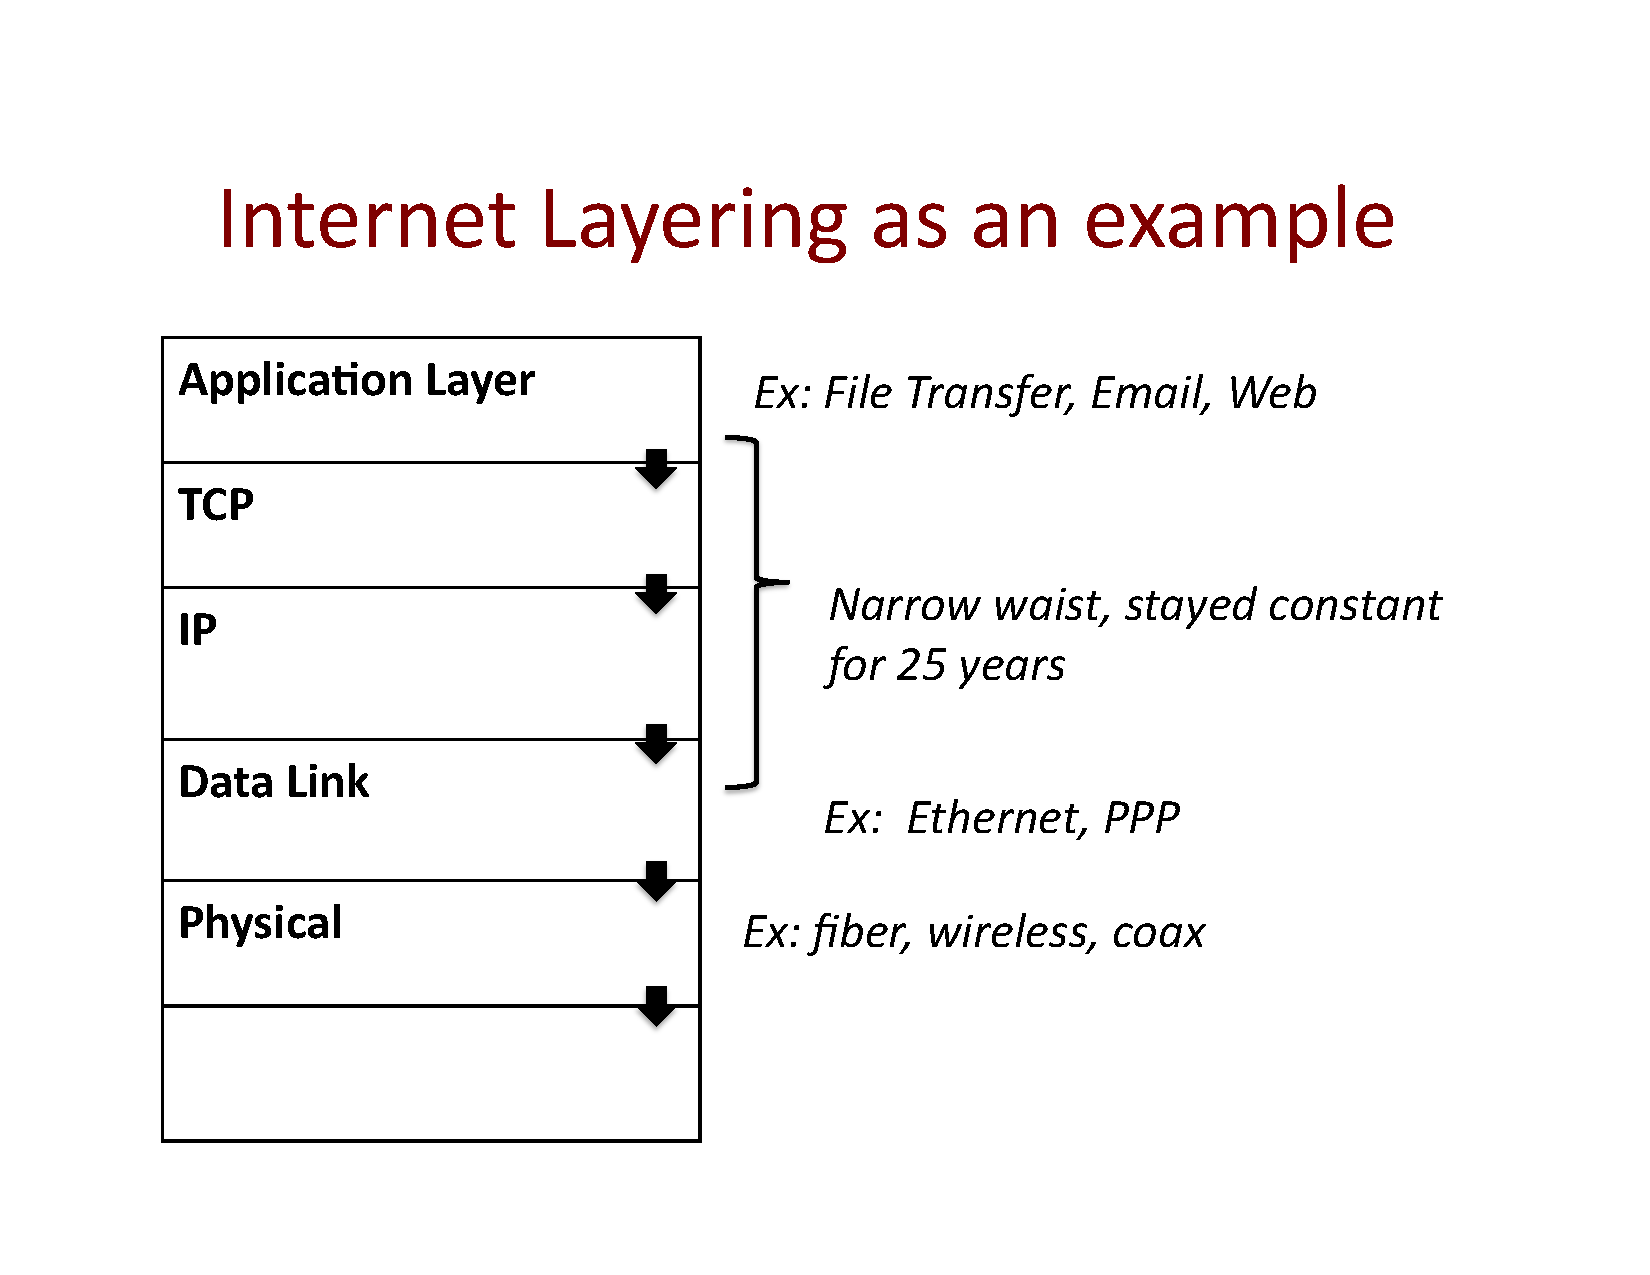
\includegraphics[width=2.75in]{fig/TCPlayer.pdf}
(b)  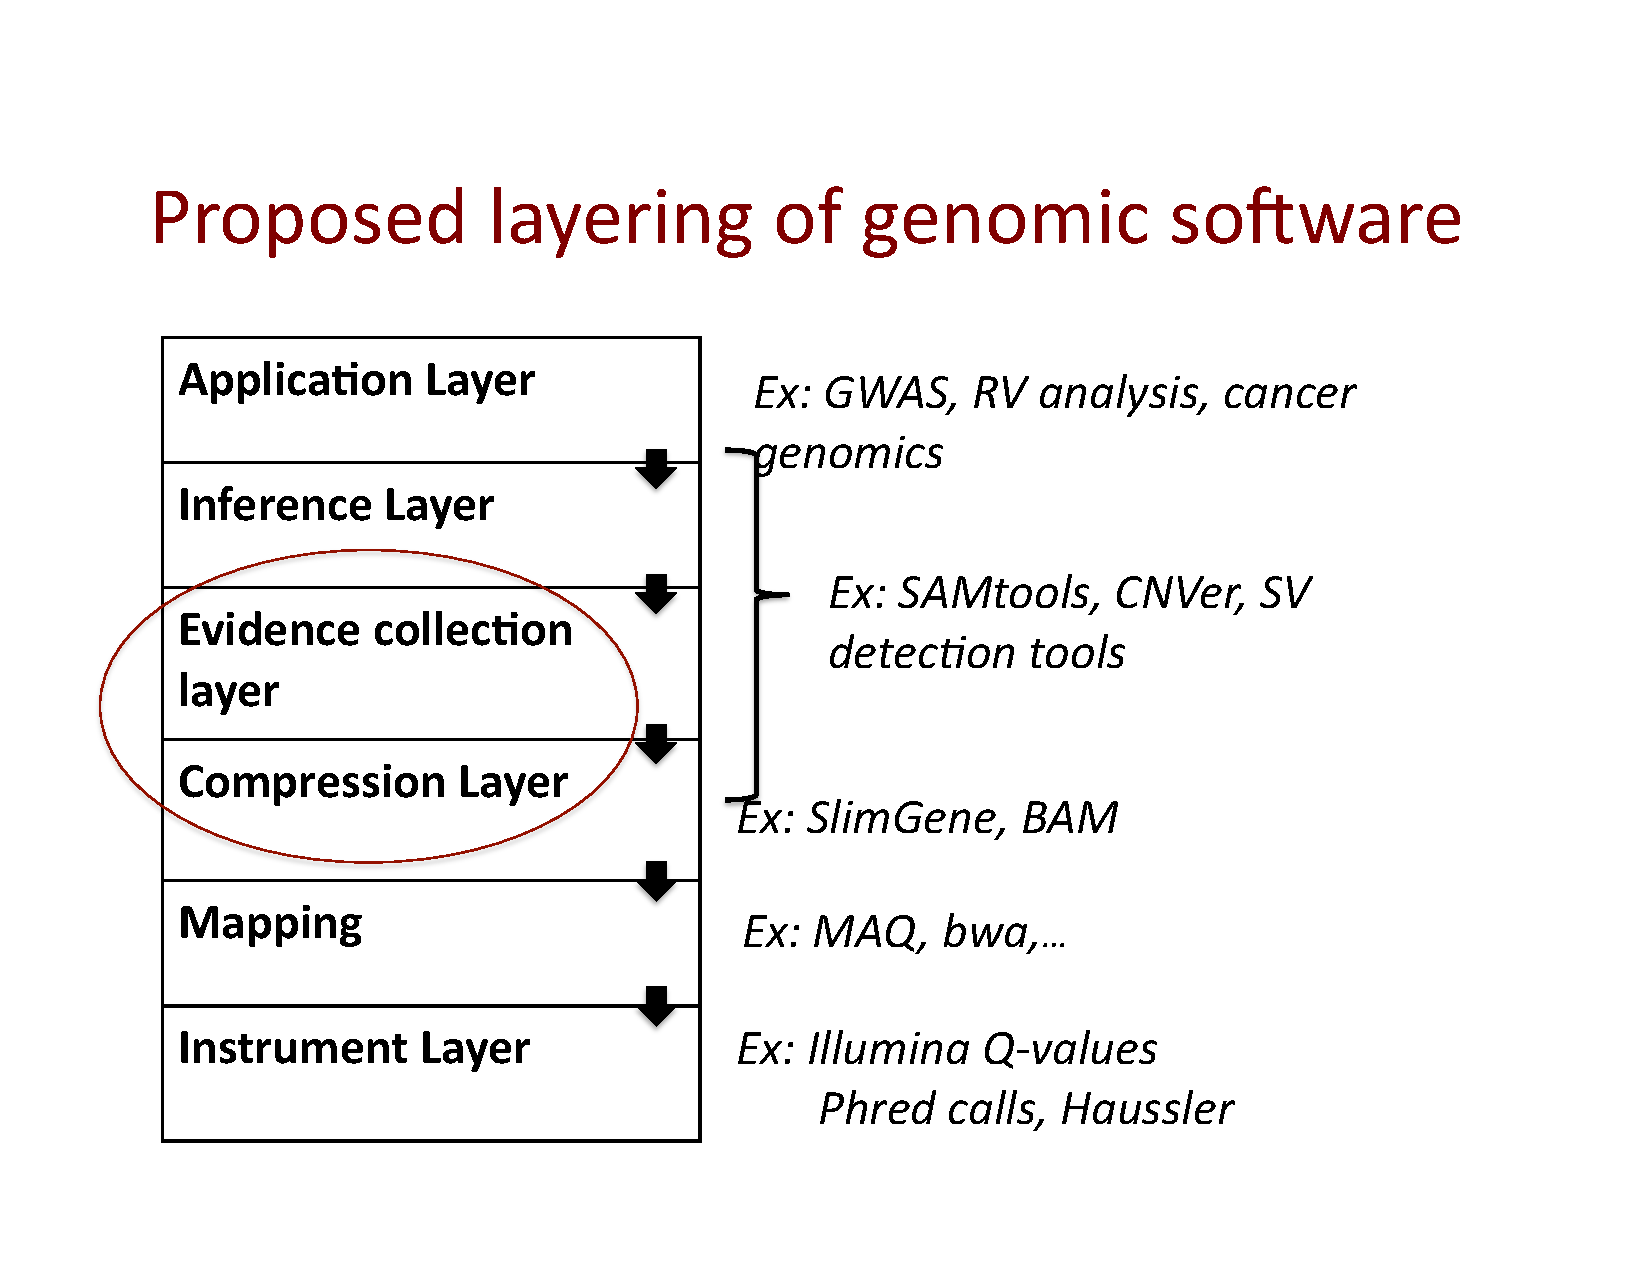
\includegraphics[width=2.75in]{fig/genomiclayer.pdf}
\caption{Layering in computer systems allowed the evelopment of
  applications like Email and Facebook without knowledge of the
  hardware (fibre/wireless) that carried traffic. A similar
  abstraction is proposed for genomics to enable the development of
  applications.}
  \label{fig:layer}
\end{figure}

Motivated by these considerations, the first part of our proposal is
an \emph{ the development of an abstraction of the genomic software
  layers that are currently in play, either explictly or implicitly}.

\section{Details: development of an abstraction for genomic queries}
A first draft of the proposed abstraction is presented in
Figure~\ref{fig:layer}b. \emph{Instrument specific software}
interprets raw instrument data (often, fluorescence signals) as
nucleotide base-pairs of genomic fragments, often with
error-profiles. These are \emph{mapped} to a standard reference, (Ex:
HG19). The mapping reveals variations, which can form the basis of new
compression schemes that store only the edits relative to the
reference, and also provide the basis for the variation catalog.

Because new sources of variation will keep being found, the
\emph{inference of variations} is therefore an important software
layer based on the mappings of donor sequences against a reference as
well as knowledge of error-profiles to help distinguish true
variations from sequencing and mapping errors. We note, however, that
each specific variation typically needs only a small portion of the
donor sequence and its mapping to the reference, and propose a new
\emph{evidence layer}, that provides this evidence upon demand. As
huge numbers of individuals are sequenced, most inference will be in
the \emph{query} mode, limited to a few genes, and a subset of the
variations. Therefore, the explicit development of the evidence layer
will help make inference more efficient. Finally, the top
layer of applications (biomedical diagnostics, pharmacogenomics, etc.)
apply the inferences to biomedical research.

We recognize that biologists will resist the aproach of abstracting
away from the raw data.  However, excessive attention to error
characteristics and other arcane details of sequencing hardware
actually limits the availability of genetic information. In
particular, as market mass moves from researchers to the clinic, we
believe this tradeoff will be acceptable if not essential. Further,
the complete information can also be provided on demand for a subset
of users. The outcome of this proposal will be a publication
describing the layering and how current bioinformatics tools fit into
the abstraction. 

\section{Details: prototype development of the compression and evidence layer}
Given the proposed layering in Figure~\ref{fig:layer}b, we argue that
the largest return on investment comes from development of the
\emph{evidence layer}. Let us return to our example of SNV
discovery. We may have two tools. Tool~A calls SNVs after loking at
alignments of reads mapped to a specific location, and the quality of
sequenced base calls. Tool~B looks at quality of mapping (is the read
mapped correctly?), and also looks at other donor sequences to see if
the SNV is known to occur in a population. Both tools use different
inferences, but rely on one basic source of \emph{evidence}: the set
of reads (possibly from a population) that map to the specified
location, and other locations in the genome where this set might map.

\subsection{EL-API: an API for the evidence layer}
\label{sec:el_api}
We will develop an EL-API to efficiently query and retrieve the raw
evidence required to make an inference. This will allow third-party
bioinformaticians to quickly develop efficient tools for inference;
They simply query our API to get the evidence, and make their
inference based on the evidence. On the other end, if Life Tech
changes instrumentation, or mapping software, they do not need to
change the EL-API, only the code supporting the EL-API.  A draft
version of the API is schematically represented in
Figure~\ref{fig:el_api}, with a more detailed description in Appendix
I. Our considerations in designing the API included the following: the
API must be (a) technology agnostic; (b) able to obtain the evidence
for all inferences regarding human variation; (c) concise, and simply
stated; and (d) allow for efficient implementation. The EL-API
automatically assumes a collection of reads mapped to a reference. For
simplicity, we assume that all reads are from a single donor
sequence. However, the API extends unchanged to a population of
individuals.
\begin{figure}[ht]
  \centering
  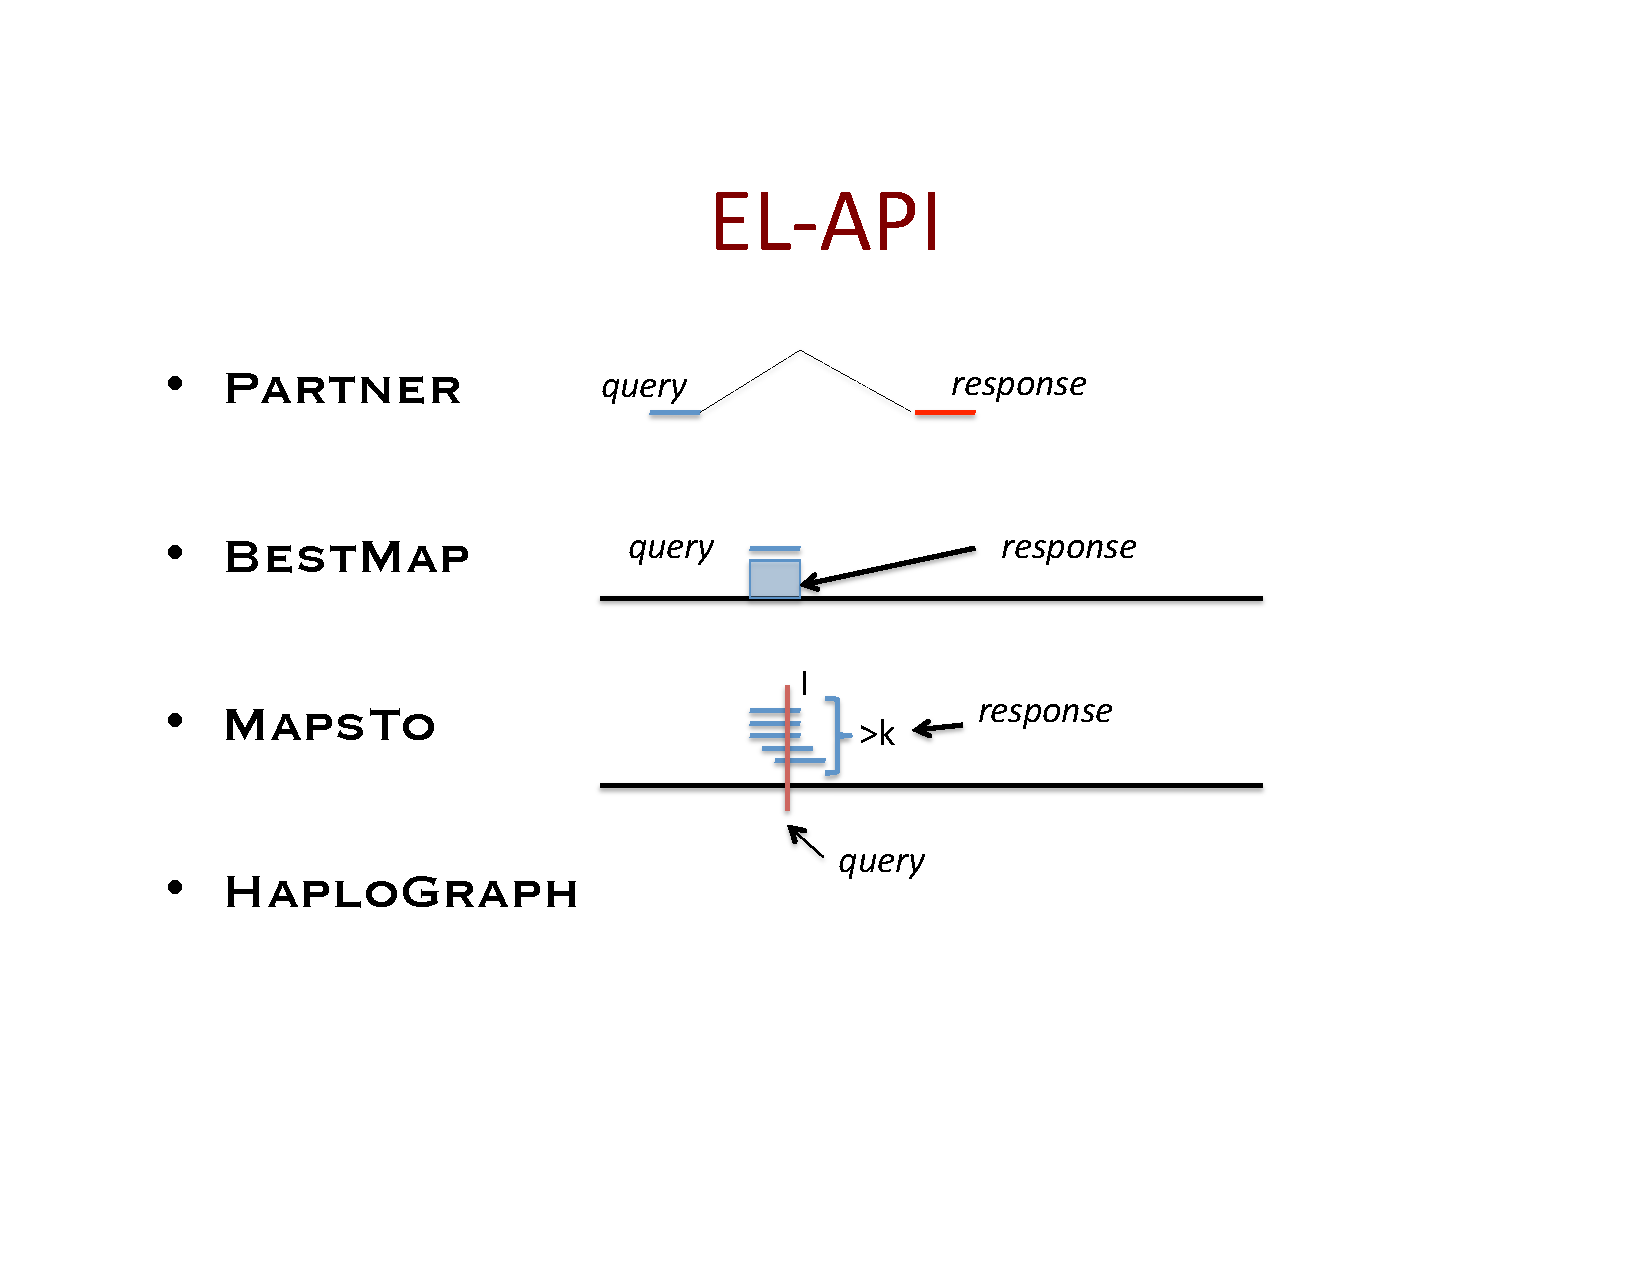
\includegraphics[trim = 25mm 50mm 40mm 20mm, clip, width=4in]{fig/ELAPI.pdf}
  \caption{A cartoon depiction of the evidence layer API.}
  \label{fig:el_api}
\end{figure}

\subsection{Development of a compression layer prototype}

To make querying more efficient, we will work with compressed
data. Our compression ideas, described in Kozanitis et al., 2010, rely
upon efficiently storing alignments of sub-reads to the
reference. This abstraction helps in EL-API. In addition, we will
develop appropriate indices and data structures to make the querying
more efficient.



\newpage

\section{ EL-API}

We start with some definitions: a \emph{read} is a DNA clone sampled
from a donor. A \emph{sub-read}, or a fragment is the part of the read
that is sequenced. A paired-end read will have two sub-reads, but
newer (strobe) reads can have multiple sub-reads.


\begin{enumerate}
\item {\sc Partner:} Given a sub-read, or a read as input, identify
  all of the sub-reads that come from the same read.
\item {\sc BestMap:} The input is a collection of reads or
  sub-reads. The output is the location of the optimal mapping of the
  sub-reads, along with an encoding of the alignment.
\item {\sc AllMaps:} The input is a collection of reads or
  sub-reads. The output is the set of multiple locations where the
  sub-reads match up, along with an encoding of the alignments.
\item {\sc MapsTo:} The input is a collection of intervals $I$. The
  output is a collection of all reads that whose bestmap alignments
  intersect with $I$.
\item {\sc Coverage:} The input is a collection of intervals $I$. The
  output is the number of reads in {\sc MapsTo} ({\bf Derived from
    MapsTo}).
\item {\sc HaploGraph:} The input is a collection of locations $S$
  corresponding to known SNVs. The output is a graph $G(S,E_S)$, where
  each edge $(u,v)\in E_S$ is labeled with reads whose sub-reads span
  both $u$ and $v$. An edge exists only of the corresponding set of
  reads is non-empty.
\item {\sc Keyword}
\end{enumerate}
\subsection{Calling SNPs:}
In order to infer the alleles at a given site, we can use {\sc MapsTo}
to identify all sub-reads that overlap, and their alignments.
\subsection{Large deletions:}
The typical questions in this case are:
\begin{description}
\item [Q1:] Does the individual have a deletion in a gene (specified
  as a collection of intervals, $I$? {\bf Ans.} Use {\sc MapsTo} to
  quickly retrieve all sub-reads that map to $I$. Return the subset of
  reads, whose partners have length-discordant mapping. The inference
  layer will also use {\sc AllMaps} to varify that the discordant
  reads are accurate.
\item [Q2:] Identify all deletions that are supported by at least $k$
  reads? {\bf Ans.} First retrieve all regions, where the {\sc
    Coverage} is at least $k$. For each such region, check if the
  reads have length-discrepant partners. Return all length-discrepant
  reads (using {\sc MapsTo}) if the coverage is at least $k$.
\end{description}

\subsection{Haplotypes:}
\begin{description}
\item [Q1:] Given two variant locations, $a,b$, and a collection of
  variant locations $S$, return the two haplotypes connecting $a,b$
  using variants in $S$. {\bf Ans.} Use {\sc HaploGraph} on $S$ to get
  a graph. Prune the graph to get the sub-graph $G'$ connecting
  $a,b$. Return $G'$ and all reads labeling its edges.

\item [Q2:] Identify all deletions that are supported by at least $k$
  reads? {\bf Ans.} First retrieve all regions, where the {\sc
    Coverage} is at least $k$. For each such region, check if the
  reads have length-discrepant partners. Return all length-discrepant
  reads (using {\sc MapsTo}) if the coverage is at least $k$.
\end{description}
\end{document}
